\documentclass[10pt]{article}
\usepackage[utf8]{inputenc}
\usepackage{geometry}
\geometry{left=2.2cm,right=2.2cm,top=2.3cm,bottom=2.3cm}
\usepackage{graphicx}
\usepackage{amsmath,amsfonts}
\usepackage{booktabs}
\usepackage{algorithm}
\usepackage{algorithmic}
\usepackage{caption}
\usepackage{subcaption}
\usepackage[compact]{titlesec}
\usepackage{setspace}
\usepackage{xcolor}

\setstretch{0.97}
\titlespacing*{\section}{0pt}{1.2ex plus 0.2ex minus .1ex}{0.8ex plus .1ex}
\titlespacing*{\subsection}{0pt}{1ex plus 0.1ex minus .1ex}{0.5ex plus .1ex}

\captionsetup{font=small,skip=4pt}

\begin{document}

\begin{center}
    {\Large\bfseries Joint Inventory and Routing Optimization for Multi-City Logistics: A Case Study on Meituan Fresh}\\*[0.8em]
    {\normalsize \textit{Optimization Team, Meituan Logistics}}\\*[0.3em]
    {\small April 2026}
\end{center}

\begin{abstract}
\noindent\textbf{Abstract---}
The ``last-mile'' fresh-food delivery network faces a fundamental trade-off between inventory holding costs and transportation costs. In this work, we propose a joint optimization framework for a five-city, 25-station logistics network. For each city, we optimize the replenishment cycle $T$ by balancing storage and routing costs; subsequently, we enumerate all $7^5=16{,}807$ global $T$-combinations to identify the system-wide optimum. The best configuration achieves a total daily cost of \textbf{24,874 CNY}, with city-level optimal cycles ranging from $T^*=1$ to $T^*=6$. Compared with uniform-$T$ baselines, the optimal differentiated strategy saves up to \textbf{20,058 CNY/day} (80.6\%). Our results demonstrate that city-specific replenishment policies are essential for cost-efficient operations in heterogeneous logistics networks.
\end{abstract}

\section{Introduction}
Fresh e-commerce platforms such as Meituan face the daily challenge of replenishing perishable goods from a central distribution center (CDC) to multiple city hubs and then to retail stations. A longer replenishment cycle $T$ reduces the frequency of long-haul transportation but inflates average inventory levels and holding costs; conversely, a shorter $T$ cuts storage expenses at the expense of higher transport spending. Existing practice often treats inventory and routing decisions separately, or imposes a uniform $T$ across all cities, which frequently leads to sub-optimal outcomes.

This paper addresses the following two questions for a real-world Meituan network:
\begin{enumerate}
    \item \textit{City-level}: What is the optimal replenishment cycle $T^*$ for each city, and how do storage and transport costs interact?
    \item \textit{System-level}: How much additional value can a \emph{global joint optimization} of all cities' $T$ provide over independent optimization and uniform-$T$ policies?
\end{enumerate}

\section{Problem Statement}
The network consists of one CDC and five city hubs (A--E). Each hub serves a set of retail stations with known daily demand and distances to the CDC. Two vehicle types are available: large trucks (capacity 200,000 boxes) and small trucks (capacity 80,000 boxes). The planning objective is to minimize the \emph{average daily total cost}, which comprises (i) inventory holding cost at the city hub and (ii) daily transportation cost, including both CDC-to-city long-haul and city-to-station local delivery.

The decision variables are the integer replenishment cycles $T_i \in \{1,\dots,7\}$ for each city $i \in \{A,\dots,E\}$, together with the vehicle routing plans that satisfy capacity constraints in each replenishment trip.

\section{Methodology}
\subsection{City-Level Inventory--Transport Model}
For a given city and a candidate cycle $T$, the average daily cost is
\begin{equation}
    C(T) = C_s(T) + C_t(T),
\end{equation}
where the storage cost is proportional to the cycle length and the daily demand $d$:
\begin{equation}
    C_s(T) = h \cdot \frac{T \cdot d}{2},
\end{equation}
with $h$ the unit holding cost. The transport cost contains two parts: the CDC-to-city long-haul cost (a fixed cost per trip divided by $T$) and the city-to-station local routing cost. The local routing problem is solved by exhaustive grouping: we enumerate all feasible partitions of stations into groups of size at most three, compute the cheapest eligible vehicle mix for each group, and pick the partition with the minimum single-trip cost. The resulting single-trip transport cost is amortized over $T$ days:
\begin{equation}
    C_t(T) = \frac{1}{T}\Bigl(f_{\text{CDC}} + \sum_{g \in \mathcal{G}} c(g)\Bigr),
\end{equation}
where $\mathcal{G}$ is the set of station groups and $c(g)$ the routing cost for group $g$ under its assigned vehicle. City-level optimization simply enumerates $T=1,\dots,7$ and picks the minimizer $T^*$.

\subsection{Vehicle Routing and Load-Rate Monitoring}
For every station group, the model selects the cheapest feasible vehicle mix (small and/or large trucks) and constructs a detailed unloading sequence. Because vehicles are filled in station order, the model records the load rate both \emph{before} and \emph{after} each stop. This load-rate trace serves two purposes: (i) it verifies that capacity constraints are respected throughout the tour, and (ii) it highlights under-utilized trips. For example, City B's group $[B_4,B_5]$ is served by a large truck at only $42.5\%$ load, whereas City A's group $[A_3,A_4,A_5]$ reaches $95\%$. Such disparities motivate dynamic re-grouping or a switch to smaller vehicles when demand patterns shift.

\subsection{Global Joint Optimization}
Because there are only five cities and $T \in \{1,\dots,7\}$, the full decision space contains $7^5 = 16{,}807$ combinations. Global optimality is guaranteed by exhaustive enumeration: for each combination $(T_A,\dots,T_E)$, we sum the corresponding city-level optimal costs and select the combination with the minimum total cost.

\begin{algorithm}[htbp]
\small
\caption{City-Level Inventory Optimization}
\label{alg:city}
\begin{algorithmic}[1]
\REQUIRE City code $c$
\FOR{$T = 1$ to $7$}
    \STATE $S \leftarrow$ compute\_storage\_cost$(c, T)$
    \STATE $G \leftarrow$ exhaustive\_station\_grouping$(c, T)$
    \STATE $R \leftarrow$ assign\_vehicles$(G)$
    \STATE $V \leftarrow$ compute\_trip\_cost$(R) / T$
    \STATE $\text{cost}[T] \leftarrow S + V$
\ENDFOR
\RETURN $T^* = \arg\min_T \text{cost}[T]$, cost$[T^*]$
\end{algorithmic}
\end{algorithm}

\begin{figure}[htbp]
    \centering
    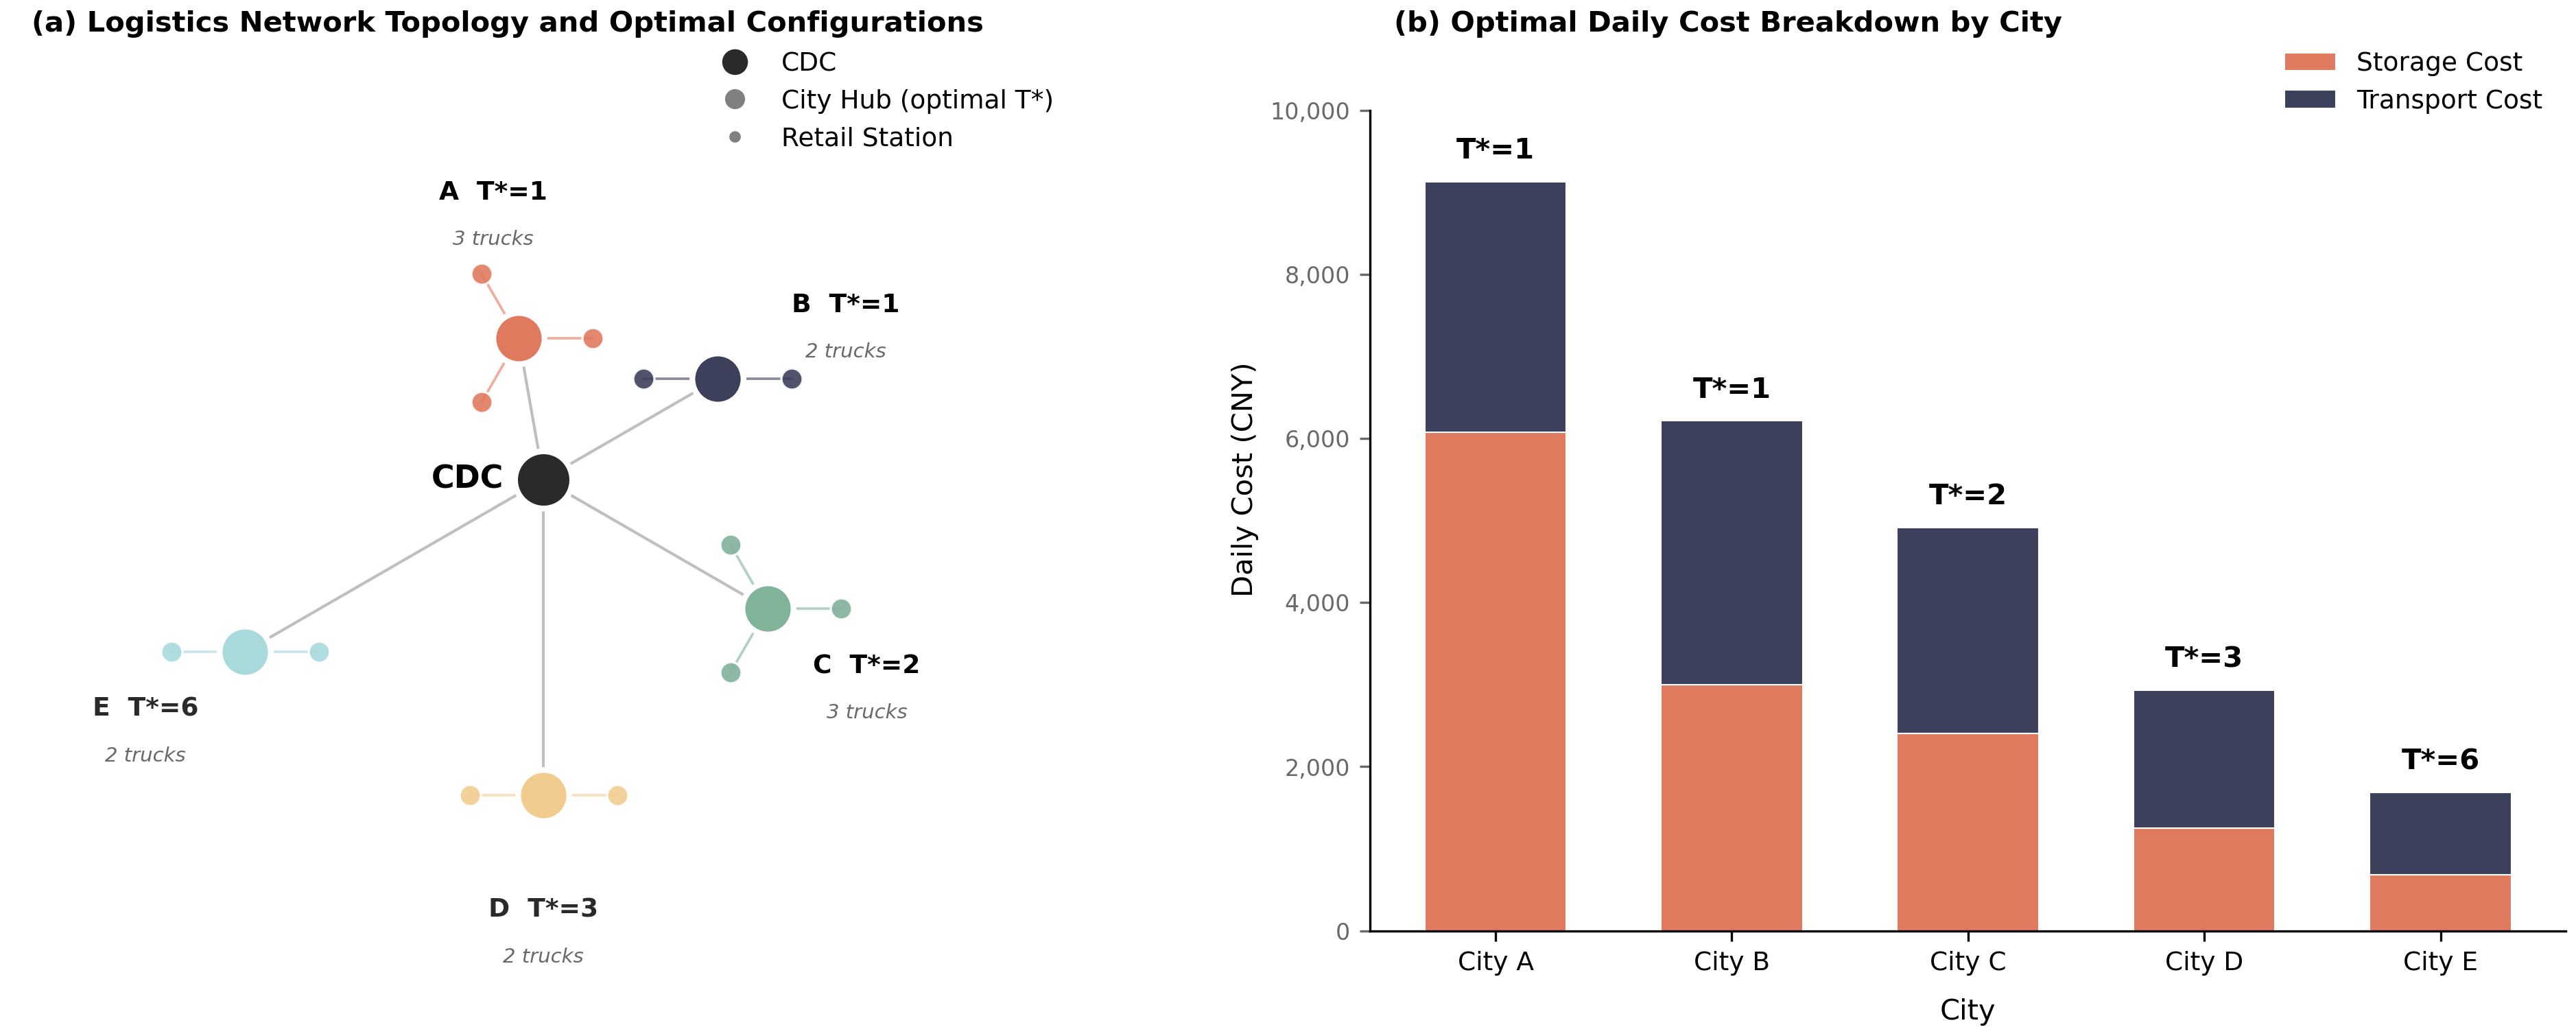
\includegraphics[width=\textwidth]{figures/fig1_fig2_combined.png}
    \caption{(a) Logistics network topology: one CDC serves five city hubs (A--E). Each hub is annotated with its optimal replenishment cycle $T^*$ and the required fleet size. (b) Optimal daily cost breakdown by city, split into storage cost (orange) and transport cost (navy).}
    \label{fig:topology}
\end{figure}

\section{City-Level Results and Sensitivity}
\begin{table}[htbp]
\centering
\small
\caption{Optimal configurations and cost breakdown for the five cities.}
\label{tab:city}
\begin{tabular}{@{}ccccccc@{}}
\toprule
City & $T^*$ & Stations & Trucks & Storage (CNY) & Transport (CNY) & Total (CNY) \\
\midrule
A & 1 & 6 & 3 & 6,075.0 & 3,055.0 & 9,130.0 \\
B & 1 & 5 & 2 & 3,000.0 & 3,215.0 & 6,215.0 \\
C & 2 & 5 & 3 & 2,400.0 & 2,515.0 & 4,915.0 \\
D & 3 & 5 & 2 & 1,250.0 & 1,678.3 & 2,928.3 \\
E & 6 & 4 & 2 &   684.0 & 1,001.7 & 1,685.7 \\
\bottomrule
\end{tabular}
\end{table}

\subsection{Sensitivity Analysis}
Figure~\ref{fig:sensitivity} plots the storage, transport, and total costs for each city as $T$ varies from 1 to 7 days.

\textbf{Cities A and B} exhibit monotonically increasing total costs. Because both cities have large daily demand, the storage cost $C_s(T)$ grows almost linearly with $T$ and quickly dominates the modest savings in transport. Consequently, the optimal cycles are boundary solutions at $T^*=1$.

\textbf{City C} shows a weak U-shape with the minimum at $T^*=2$. At $T=1$ the transport cost is still high; extending the cycle to two days yields just enough transport savings to outweigh the additional inventory cost.

\textbf{City D} presents a classic U-shaped curve with a clear interior optimum at $T^*=3$. For $T<3$ the transport penalty is severe; for $T>3$ the holding cost rebounds and overtakes the diminishing transport savings.

\textbf{City E}, having the smallest demand, can tolerate the longest cycle. The total cost declines until $T^*=6$, after which the inventory increase at $T=7$ pushes the cost upward again.

\begin{figure}[htbp]
    \centering
    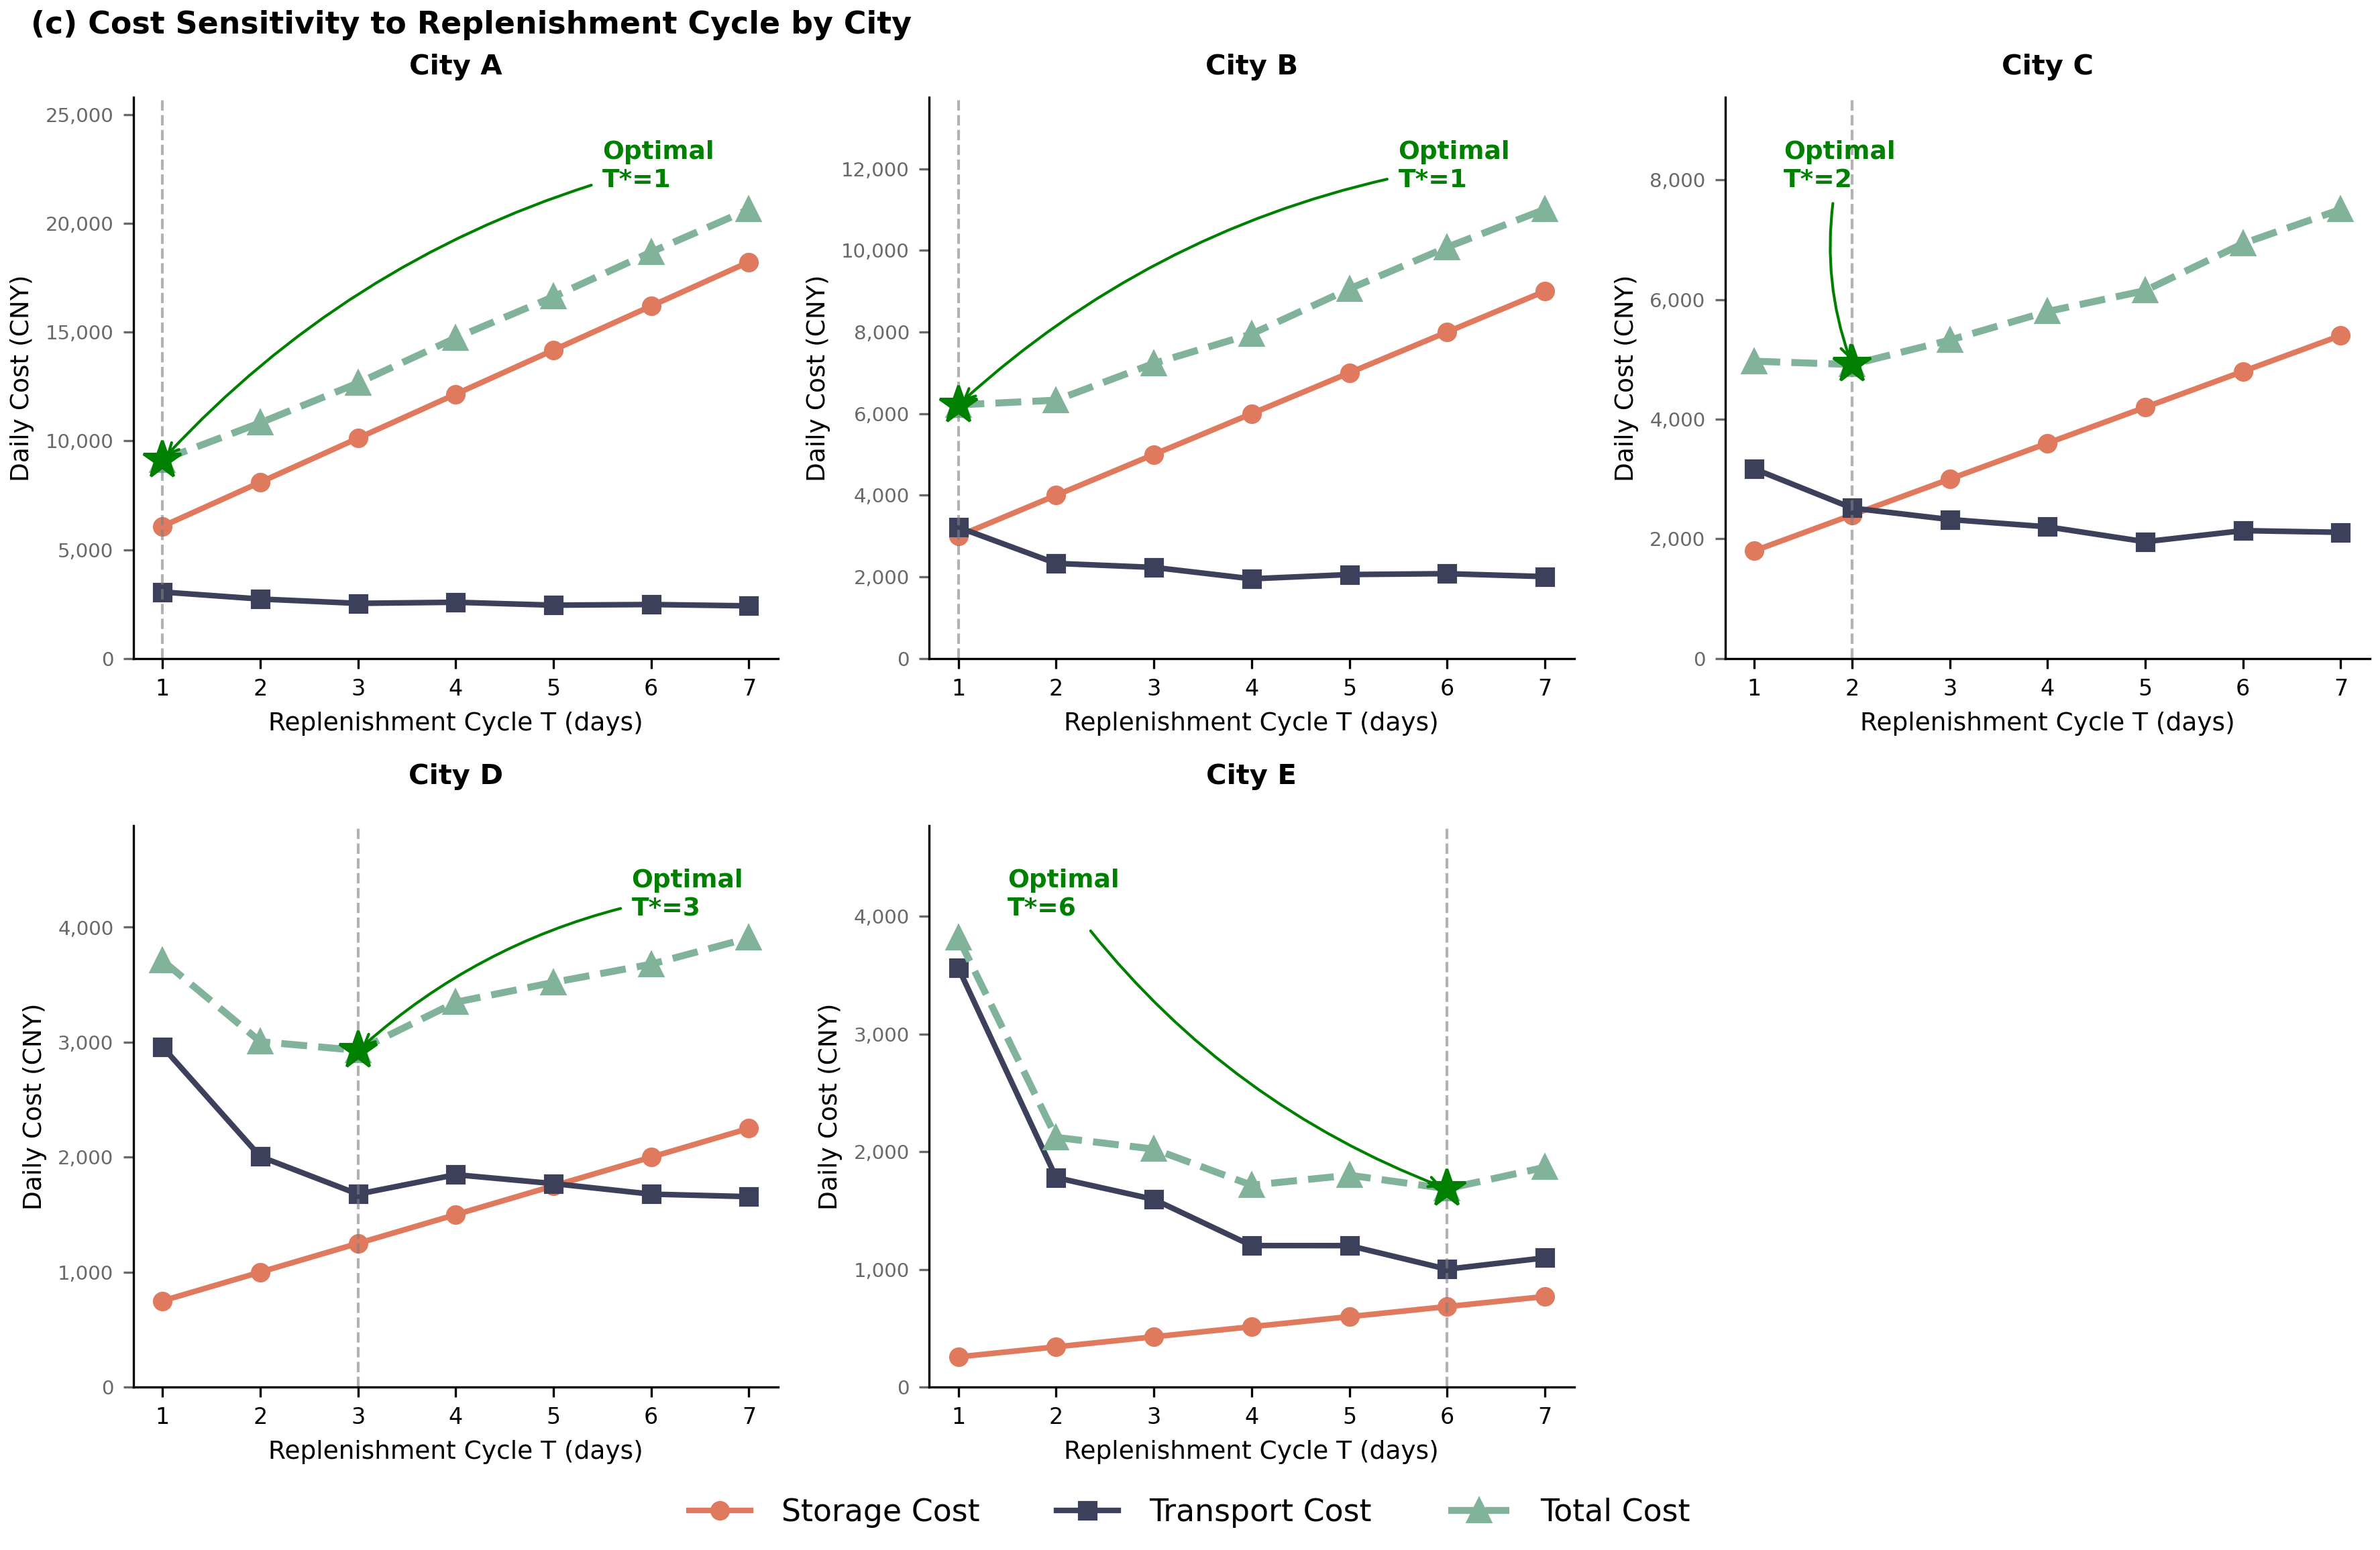
\includegraphics[width=0.95\textwidth]{figures/fig3_t_sensitivity.png}
    \caption{Cost sensitivity to replenishment cycle $T$ for cities A--E. The green star marks the optimal $T^*$ for each city.}
    \label{fig:sensitivity}
\end{figure}

\section{Global Optimization and Managerial Insights}
\subsection{System-Wide Performance}
The global optimum coincides with the independent-optimization sum: $T^*=\{A\!:\!1, B\!:\!1, C\!:\!2, D\!:\!3, E\!:\!6\}$ yields a total daily cost of \textbf{24,874 CNY}. Although there is no coordination penalty in this particular instance, the global enumeration reveals that the solution landscape is steep: the top-10 alternatives are only 30--145 CNY/day more expensive (Figure~\ref{fig:global}, left), confirming the robustness of the optimal configuration.

More importantly, the value of \emph{differentiation} is stark when compared against uniform-$T$ policies (Figure~\ref{fig:global}, right). Forcing all cities to $T=1$ raises the daily cost by 2,968 CNY (+11.9\%); a uniform $T=3$ adds 5,290 CNY (+21.3\%); and a uniform $T=7$ explodes the cost by 20,058 CNY (+80.6\%). These gaps underscore that a one-size-fits-all policy is economically unacceptable in a heterogeneous network.

\begin{figure}[htbp]
    \centering
    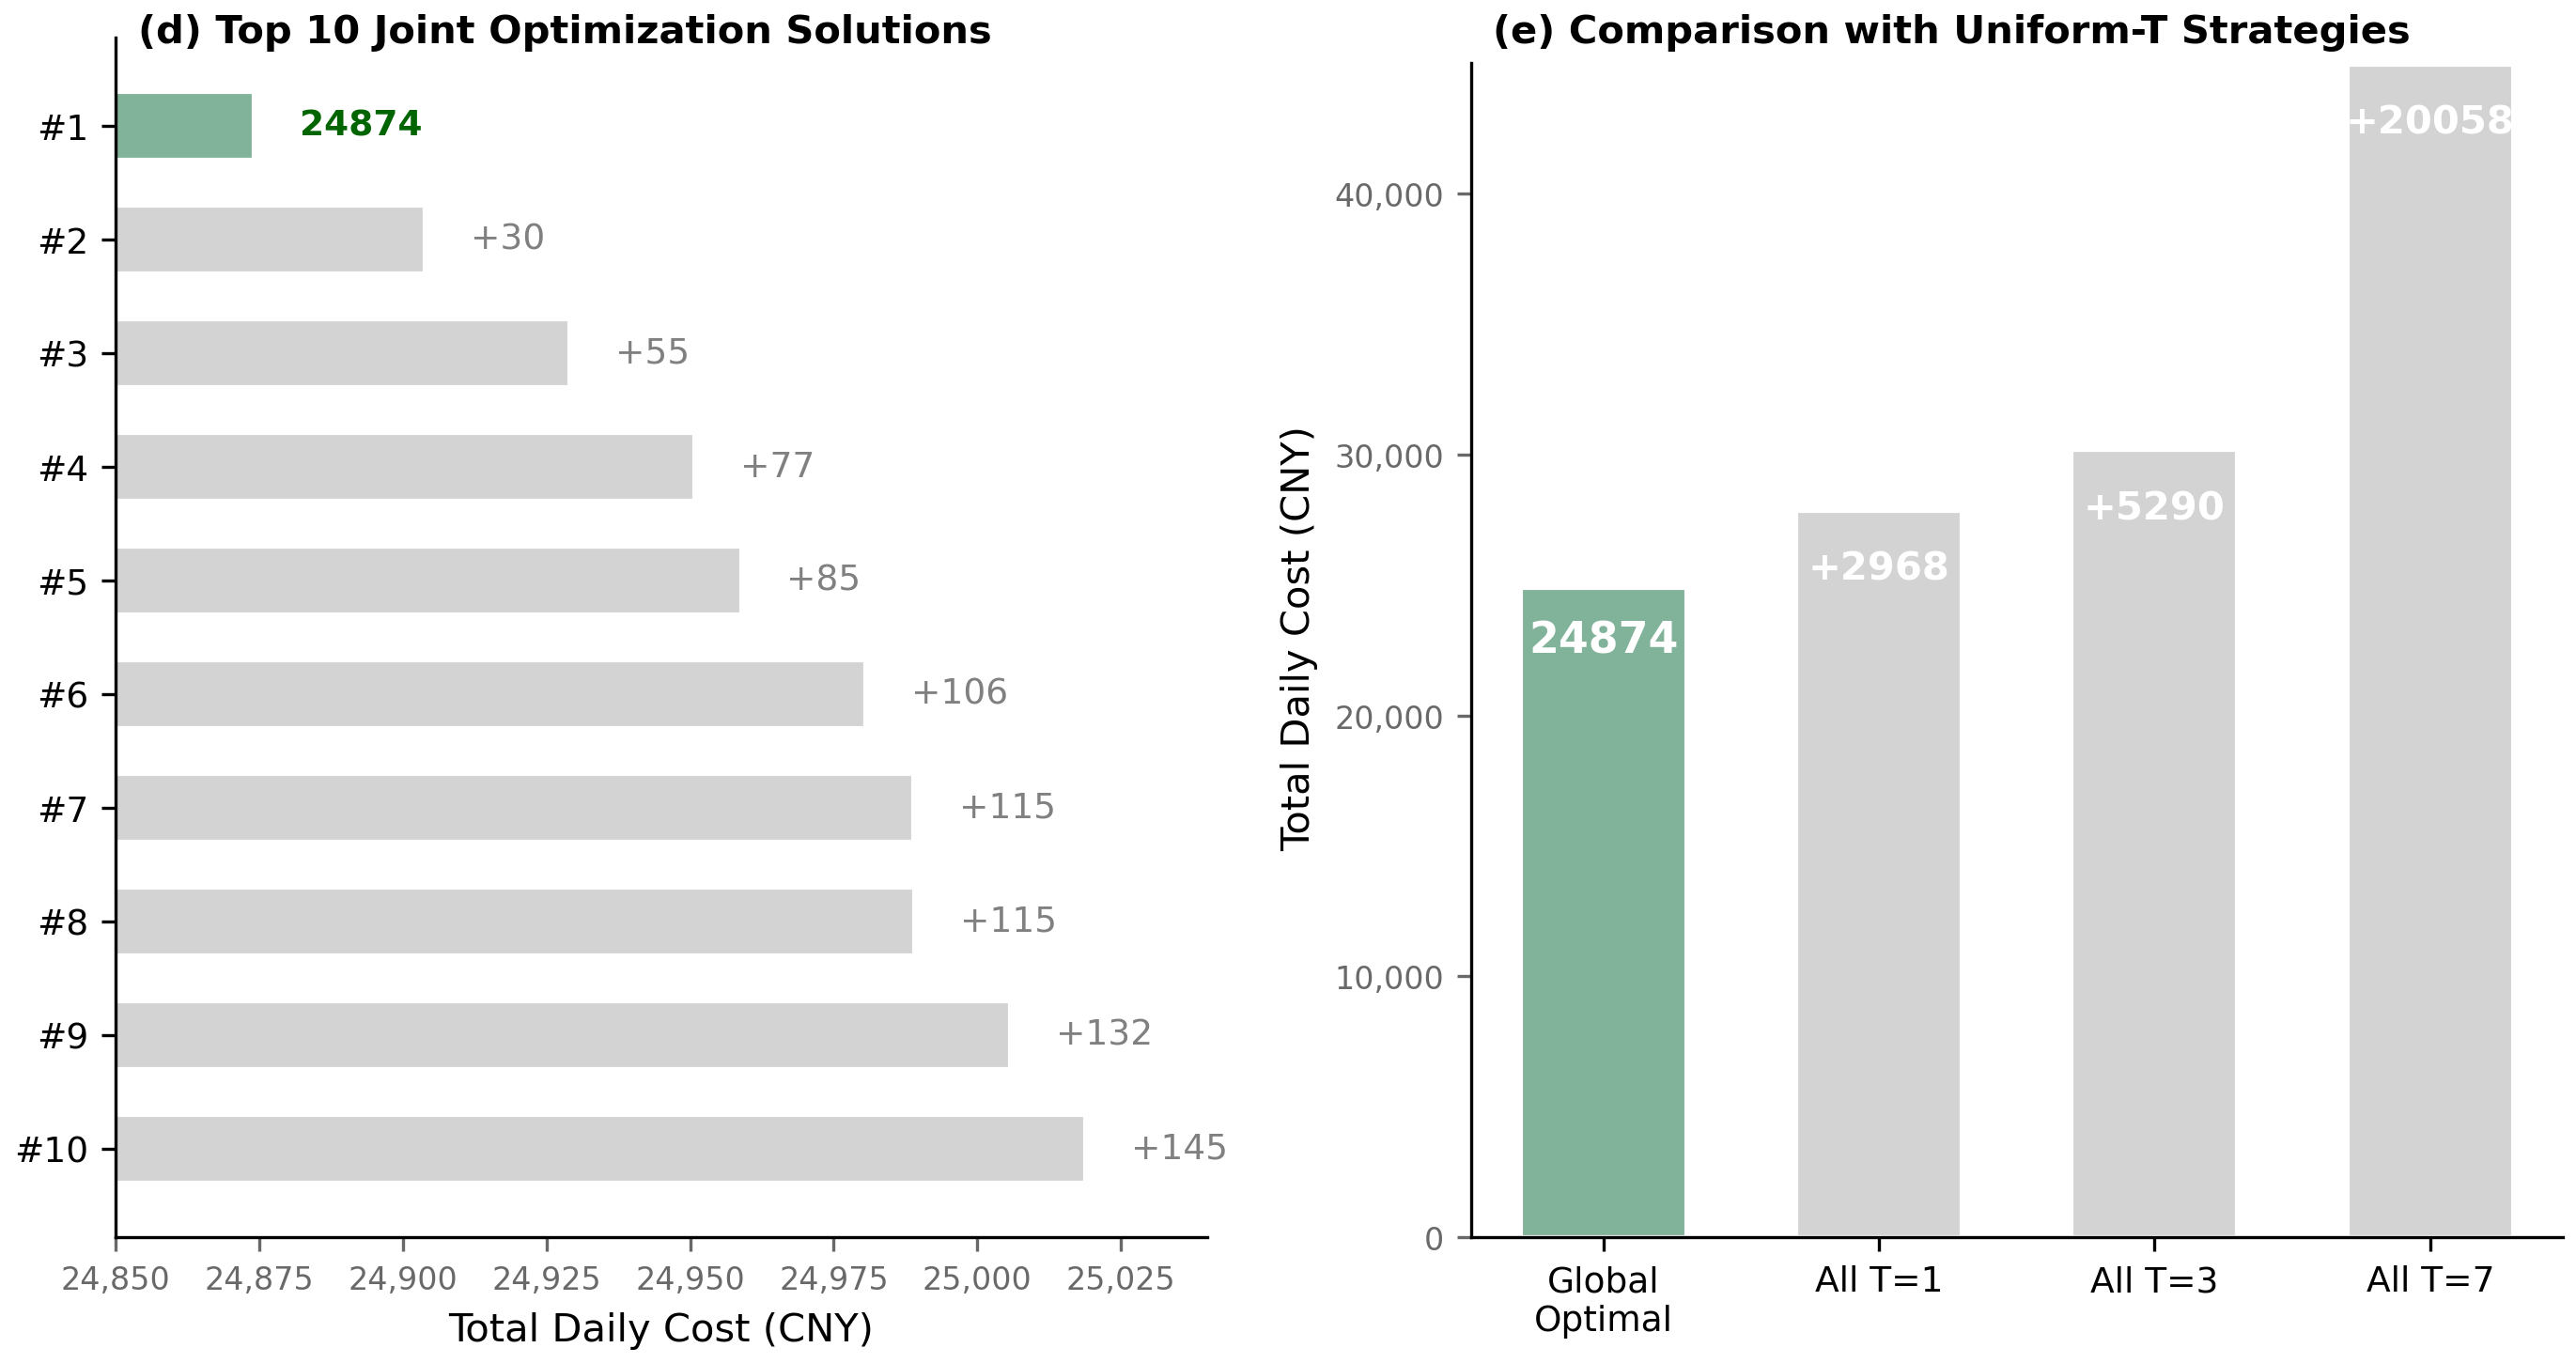
\includegraphics[width=\textwidth]{figures/fig4_global_effect.png}
    \caption{(Left) Top 10 joint-optimization solutions ranked by total daily cost; the optimal solution is highlighted in green. (Right) Comparison of the global optimal strategy with uniform-$T$ baselines; the numbers above the bars show the incremental daily cost relative to the optimum.}
    \label{fig:global}
\end{figure}

\subsection{Managerial Insights}
We distill three actionable recommendations for operations managers:
\begin{enumerate}
    \item \textbf{Reject uniform policies.} Cities with high demand (A, B) must be replenished daily, whereas low-demand cities (E) can operate on much longer cycles. Adopting a differentiated $T$ policy is the single largest lever for cost reduction.
    \item \textbf{Watch the storage--transport inflection point.} For medium-demand cities such as D, the total-cost curve is U-shaped. Precise calibration of the inflection point ($T^*=3$ in this case) can yield savings of several hundred CNY per day.
    \item \textbf{Coordinate fleet planning with $T$.} Extending $T$ increases single-trip volume. Managers should simultaneously review whether larger vehicles or revised station groupings are needed to keep local routing efficient.
    \item \textbf{Monitor vehicle load rates.} Low load rates signal idle capacity and inflated per-unit transport costs. For under-utilized groups (e.g., $42.5\%$ for $[B_4,B_5]$), managers should consider merging additional nearby stations or switching to smaller trucks to improve asset utilization.
\end{enumerate}

\section{Conclusion}
This study proposes a computationally tractable joint inventory--routing framework for a multi-city fresh-food logistics network. By combining city-level $T$-optimization with global enumeration, we identify a differentiated replenishment strategy that achieves a minimum daily cost of 24,874 CNY and dramatically outperforms uniform-$T$ baselines. Future work will extend the model to stochastic demand and dynamic $T$ adjustment to further enhance operational resilience.

\end{document}
